\scanpage{98}
% archive sheet number: 97
quelconque. \mbox{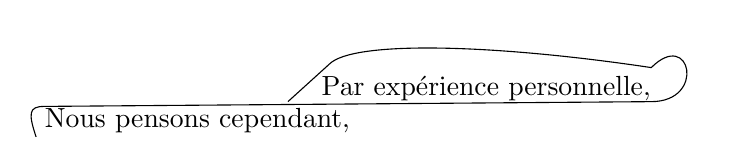
\begin{tikzpicture}[baseline=(base.base)]
\node[inner sep=0] (base) {Nous pensons cependant\deleted{,}};
\node[anchor=south west,inner sep=0,xshift=10em,yshift=.5ex] (added) at (base.north west) {\inserted{Par expérience personnelle,}};
\draw ([xshift=-.3em,yshift=-.3ex]base.south west) .. controls +(-.1,.3) and +(-.2,0) .. ([yshift=.1ex]base.north west) -- (added.south east) .. controls +(.7,0) and +(.5,.5) .. ([yshift=.7ex]added.north east) .. controls +(-2,.3) and +(.3,.3) .. ([xshift=.3em,yshift=1ex]added.north west) -- ([xshift=-1.2em]added.south west);
\end{tikzpicture}} que la compréhension\deleted{, heuristique quoique pour le moment largement heuristique,} obtenue grâce aux arguments de poids et de niveaux, quoiqu'elle soit pour l'instant entièrement heuristique, \deleted{est et} peut être la source de la découverte de propriétés importantes et inattendues pour la cohomologie des variétés algébriques, \deleted{même si} et qu'elle mérite pour cette raison de ne pas être dédaignée. De plus, dans le cas des corps de caractéristique nulle, \deleted{des travaux récents fort remar les magnifiques t} le ré\rlap{\deleted{\unsure{a|c}}}\handwritten{c}ent et magnifique travail de P. DELIGNE sur la théorie de \mbox{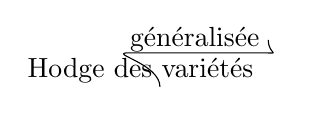
\begin{tikzpicture}[baseline=(base.base)]
\node[inner sep=0] (base) {Hodge des variétés};
\node[anchor=south west,inner sep=0,xshift=3.7em,yshift=.4ex] (added) at (base.north west) {\inserted{généralisée}};
\draw ([xshift=4.8em,yshift=-.3ex]base.south west) .. controls +(0,.3) and +(-.3,0) .. (added.south west) -- (added.south east) .. controls +(.3,0) and +(0,-.2) .. ([xshift=.3em]added.east);
\end{tikzpicture}} algébriques quelconques sur le corps $\underline{C}$ des nombres complexes\deleted{,} \mbox{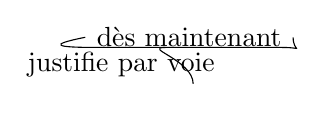
\begin{tikzpicture}[baseline=(base.base)]
\node[inner sep=0] (base) {justifie par voie};
\node[anchor=south west,inner sep=0,xshift=2.5em,yshift=.4ex] (added) at (base.north west) {\inserted{dès maintenant}};
\draw ([xshift=-.4em]added.west) .. controls +(-.5,-.1) and +(-.5,0) .. (added.south west) -- (added.south east) .. controls +(.3,0) and +(0,-.2) .. ([xshift=.4em]added.east);
\draw ([xshift=6em,yshift=-.5ex]base.south west) .. controls +(0,.3) and +(-.3,0) .. ([xshift=2.5em]added.south west);
\end{tikzpicture}} transcendante le ``yoga'' des poids et niveaux dans le cadre de la cohomologie de De Rham\handwritten{\unsure{,}} (tout en ouvrant à la théorie cohomoligue \mbox{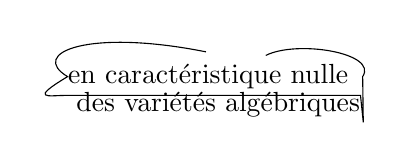
\begin{tikzpicture}[baseline=(base.base)]
\node[inner sep=0] (base) {des variétés algébriques};
\node[anchor=south west,inner sep=0,xshift=-.3em,yshift=.2ex] (added) at (base.north west) {\inserted{en caractéristique nulle}};
\draw ([xshift=5em,yshift=1ex]added.north west) .. controls +(-1.5,.3) and +(-.5,.3) .. (added.west) .. controls +(-.5,-.3) and +(-.2,0) .. ([xshift=-.4em,yshift=-.3ex]base.north west) -- ([yshift=-.3ex]base.north east) -- ([xshift=.1em,yshift=-.4ex]base.south east) -- ([xshift=.5em]added.east) .. controls +(.2,.3) and +(.4,.2) .. ([xshift=-3em,yshift=.7ex]added.north east);
\end{tikzpicture}} des voies entièrement nouvelles). Il \mbox{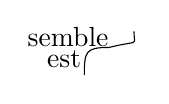
\begin{tikzpicture}[baseline=(old.base)]
\node[inner sep=0] (old) {\deleted{est}};
\node[anchor=south west,inner sep=0,xshift=-.7em,yshift=.2ex] (added) at (old.north west) {\inserted{semble}};
\draw ([xshift=.1em,yshift=-.6ex]old.south east) .. controls +(0,.3) and +(-.3,0) .. (added.south east) .. controls +(.4,.1) and +(0,-.2) .. ([xshift=.9em,yshift=.5ex]added.east);
\end{tikzpicture}} probable d'autre part que pour le cas des \deleted{Pour terminer cette introduction} variétés alg\rlap{\deleted{b}}\handwritten{é}\rlap{\deleted{\unsure{é|b}}}\handwritten{b}\rlap{\deleted{\unsure{u|r}}}\handwritten{ri}qu\deleted{p}es sur les corps de caractéristique non nulle, une justification de ce même yoga doive attendre la \mbox{
\begin{tikzpicture}[baseline=(old.base)]
\node[inner sep=0] (old) {\deleted{résolution}};
\node[anchor=south west,inner sep=0,yshift=.1ex] at (old.north west) {\inserted{preuve}};
\end{tikzpicture}} des conjectures de Weil (ou mieux, des ``conjectures standart'' de \handwritten{[\quad]}).

Pour \deleted{signaler c} terminer cette introduction, signalons que les filtrations par poids et niveaux des espaces de cohomologie $\handwritten{\ell}$-adiques, pour $\handwritten{\ell}$ variable, sont certainement relié\rlap{\handwritten{e}}\deleted{\unsure{s}}\handwritten{s} entre elles de la façon habituelle, \mbox{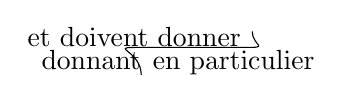
\begin{tikzpicture}[baseline=(old.base)]
\node[inner sep=0] (old) {\deleted{donnant}};
\node[anchor=base west,inner sep=0,xshift=.4em] (base) at (old.base east) {en particulier};
\node[anchor=south west,inner sep=0,xshift=-.5em,yshift=.2ex] (added) at (old.north west) {\inserted{et doivent donner}};
\draw ([yshift=-.4ex]old.south east) .. controls +(0,.3) and +(-.3,0) .. (added.south) -- (added.south east) .. controls +(.4,0) and +(0,-.2) .. ([xshift=.4em,yshift=.5ex]added.east);
\end{tikzpicture}} des espaces vectoriels sur $\underline{Q}_{\handwritten{\ell}}$ \rlap{\deleted{e}}\handwritten{d}ont le \deleted{ran} rang est indépendant de $\handwritten{\ell}$. En termes de la théorie conjecturale des motifs (suspendue entre autres aux ``conjectures standart'' déjà mentionnées), ceci devrait s'exprimer par le fait que les structures de poids \mbox{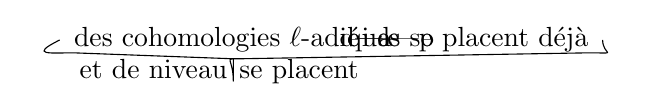
\begin{tikzpicture}[baseline=(base.base)]
\node[inner sep=0] (base) {et de niveau};
\node[anchor=base west,inner sep=0,xshift=.4em] (old) at (base.base east) {\deleted{se placent}};
\node[anchor=south west,inner sep=0,xshift=-.2em,yshift=.5ex] (added) at (base.north west) {\inserted{des cohomologies $\handwritten{\ell}$-ad\rlap{\deleted{\unsure{d|l}}}\handwritten{i}\rlap{\deleted{\unsure{é|e}}}\handwritten{q}\rlap{\deleted{i}}\handwritten{u}\rlap{\deleted{\unsure{a|p}}}\handwritten{e}s se placent déjà}};
\draw ([xshift=-.5em]added.west) .. controls +(-.4,-.2) and +(-.3,0) .. (added.south west) -- ([xshift=.2em]base.north east) -- ([xshift=.2em,yshift=-.2ex]base.south east) .. controls +(0,.3) and +(-.2,0) .. (old.north west) -- (added.south east) .. controls +(.4,0) and +(0,-.2) .. ([xshift=.5em]added.east);
\end{tikzpicture}} au niveau de\deleted{\unsure{s motifs|motifs} déjà,} la \uline{cohomologie} \deleted{des} \uline{motivique}, \mbox{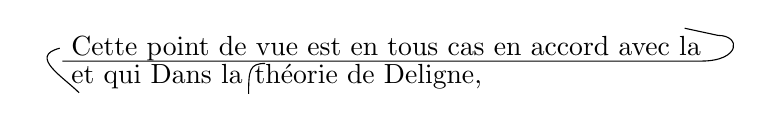
\begin{tikzpicture}[baseline=(old.base)]
\node[inner sep=0] (old) {\deleted{et qui Dans la}};
\node[anchor=base west,inner sep=0,xshift=.4em] (base) at (old.base east) {théorie de Deligne,};
\node[anchor=south west,inner sep=0,yshift=.2ex] (added) at (old.north west) {\inserted{Cet\deleted{te} point de vue est en tous cas en accord avec la}};
\draw ([xshift=-.4em]added.west) .. controls +(-.4,-.1) and +(-.2,.2) .. ([xshift=.3em,yshift=-.3ex]old.south west);
\draw ([xshift=-.3em]added.south west) -- (added.south east) .. controls +(.5,0) and +(.3,0) .. ([xshift=.6em]added.north east) -- ([xshift=-.6em,yshift=.6ex]added.north east);
\draw ([xshift=.2em,yshift=-.4ex]old.south east) .. controls +(0,.3) and +(-.2,0) .. ([xshift=.8em]old.north east);
\end{tikzpicture}} \deleted{\unsure{car}} puisque sa ``filtration par le poids'' de la cohomologie de De Rham provient d'une filtration de la cohomologie à coefficients \uline{rationnels}\handwritten{.}\deleted{(et non seulement}
